\section{Introduction}

A time series is a sequence of values, measured at regular intervals over time. The motivation of time series analysis lies in the assumption that what happened in the past has an influence on what will happen in the future. Typically, time series are used for trends analysis and forecasting future values when there are good reasons to suspect the existence of cycles in the data; for instance, a time series analysis could be used to predict the number of passengers going through Canadian airports at various points in the future. An economist might be interested in forecasting the stock market, using time series analysis. Generally speaking, the forecast horizon is the length of the prediction period: predictions at shorter horizons tend to be more reliable and accurate than predictions at longer horizons.

Ideally, the reporting periods used in time series analysis should be identical (e.g. daily, monthly, quarterly or yearly), the measurements should be taken over discrete (exclusive), consecutive periods, and the concepts and the measurement approach should be consistent over time. Detection of periodicity should be done by graphical representation of the data (and the frequency of data collection) using logic (e.g., is there an expectation of hourly, weekly, monthly, quarterly, and/or x-year cycles).

Many traditional statistical methods assume that observations are independently and identically distributed, which is unlikely to happen in real life. At best, this assumption may be sufficiently accurate to allow for some predictive power; at worst, it can lead to wildly inaccurate insights and predictions. Figure~\ref{fig:example} illustrates some examples of time series data. 
\begin{figure*}[t]
\centering
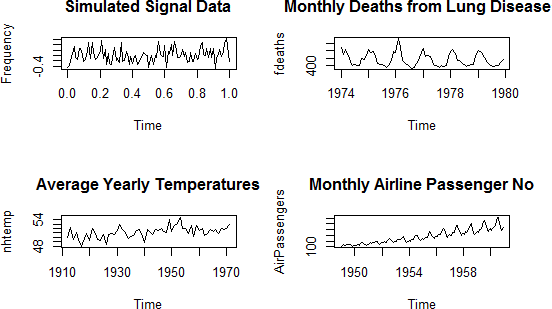
\includegraphics[width=0.81\textwidth]{Images/Example.png}
\caption{Examples of time series}\hrule
\label{fig:example}
\end{figure*}
Various time series analysis methods and tests are found in applications and in the literature, including \textit{Auto-Regressive} models (AR), \textit{Smoothing and Filtering} models (such as \textit{Moving Averages} (MA) and \textit{Exponential Smoothing} (ES)), and various other \textit{Detrending} models (ARMA, cubic splines, finite differences, etc.), \textit{Seasonal Decomposition} models (such as the \text{X11}, \text{X12}, \text{X13} and ARIMA models), and various linear and non-linear forecasting models (\textit{Holt's Method}, \textit{Winter's Method}, GARCH models, etc.). This list only skims the surface of available methods. A sample of these methods will be discussed here.

\section{Automated Trend Extraction \& Forecasting} 
Trend extraction is the detection of components within time series that can be combined in order to define the time series. Ideally, trend extraction should not be automated. There are ways to program methods (such as proc X12 in SAS or R) to automatically select the model (additive, multiplicative, etc.), to search for outliers and level shifts, etc., but the tests that are used are NOT perfect and visual examination is typically needed to confirm the procedure's decisions. That being said, it is possible to provide an algorithm that one would expect to de-trend and de-seasonalize a time series most of the time (the caveat being that unless one verifies the results on a given time series, one cannot be sure that the assumptions built into the algorithms apply to that time series). MATLAB has a time series module; some of the documentation gives suggestions as to how to automate trend extraction. But MATLAB is not a native time-series environment: SAS or R are preferred alternatives. Algorithms can be prepared once specific time series are exhibited. 

Forecasting, is different from modeling the trend of the exist data. A good fitting model (or robust model, statistically speaking) is not necessarily good at forecasting. 
\textbf{Short-term forecasting:}  There is no standard strategy or theory that can answer the question of how few observations can be used to build a model. It depends on the number of estimated parameters and also on how random the data is. With some methods, such as least squares estimation, it is feasible to create a model if the number of observation is greater than the number of estimated parameters. Some other approaches, such as LASSO, also allow analysts to build models with fewer observations than the parameters. 
\textbf{Long-term forecasting:}  Due to the nature of real data, not generated from any models, ARIMA does not perform well on long-term forecasting, and neither do other approaches. With too much data, the amount of randomness and computational complexity increases, and thus forecasting is no longer effective and also time-consuming. To solve this issue, non-parametric models are more robust than parametric models, which take time-changing into consideration -- that is, the earliest observation becomes the least important in the forecasting model. 

Thus, automated trend extraction and forecasting is to some extent possible, but there is a high probability that the resulting automated system will make mistakes. To avoid misleading users of the automated system:
 \begin{itemize}[noitemsep]
\item The results generated by the automated system should be audited by people from time-to-time
\item Metrics should be generated to convey the confidence that can be placed on the results produced by the automated system
\item There must be a consideration of the cost that will be incurred if the automated system produces ``wrong'' results
\end{itemize}

\section{Data Pre-Processing Strategies}

Ideally, in time series analysis, we have ``rectangular'' data -- each record having the same number of observation at each time step. In real situations, however, missing data is a very common and significant feature of the dataset. For that reason, the first attempt at solving the missing data problem is to impute these values (i.e. provide values for missing data), instead of removing them all (one exceptional case is when the 
  Recompile
data is sufficient and the missing data is limited -- in this situation removing the missing cases could also be practical). Last observation carried forward, mean imputation, regression imputation and multiple imputation are all simple and effective approaches to replace the missing data. Analysts need to be cautious of this step since imputed values cannot add new knowledge to the dataset which was not originally present in the dataset. Furthermore, imputation can add bias to the data if not done properly. Outright removal (list deletion) should NOT be considered, as this can introduce bias from which the experiment simply cannot survive. 
 
Multiple imputation extracts useful information from the available observations by completing the dataset (in potentially different ways) a number of times (typically 5-10). Analyses can then be run on each complete dataset, and the results are combined statistically: the estimates incorporate the uncertainty found in the dataset. This works well for up to 30-40 variables, but is poorly suited to datasets with endemic missing values. There exists software that can help with multiple imputation, notably Amelia. Certain time series methods also work with missing values (X12 in SAS or R, the Kalman filter); others do not. MATLAB's getdatasamples method allows the user to re-sample a time series at missing values (using various interpolation methods). When time series values are missing systematically or in large number, the problem of imputation may reduce to a problem of forecasting.  

\textbf{Missing imputation for data streams}: the imputation approaches discussed above are not practical for streamed data, which is often incoming at a high frequency, for the following reasons: a) the statistical methods do not specify how much information analysts should know about the data environments; b) the similarities between different completed cases are very difficult to extract, and it is possible that one data stream is completely different from its neighbours; c) it is time consuming when analysts try to use all the available information to estimate the missing values, especially when the missing data is less relevant to the known information d) missing data may or may not appear at random, which requires analysts to obtain the property of the missing values first, in order to apply any statistical analysis. 

Nan Jiang and Le Gruenwald proposed an estimation technique, using associating rule mining on streaming data based on closed frequent itemsets (CARM), and validated their approach by comparing the performance between their method to other techniques, including Window Size (AWS), the Simple Linear Regression (SLR), the Curve Regression (CE), and Multiple Regression (MR). The results generated from CARM were more accurate.  

\section{Parameter Estimation}

In the case of parametric algorithms, an assumption is made in advance about the structure of the model that can best be applied to the data (i.e. which model is most appropriate). The chosen model will then have particular parameters, the number and nature of which are pre-defined based on the model choice. The values of these parameters are then estimated according to a best fit strategy. In this case, if an incorrect assumption is made about which model is best suited to the data, then the model may fail to fit the data well, regardless of how the parameter values are varied. Non-parametric models make few structural assumptions and thus have fewer constraints with respect to the number and nature of the model parameters themselves- in this case, the selection of these, as well as the values assigned to the parameters, are driven by the nature of the data itself.

We are going to discuss parameters setting for some selective non-parametric algorithms in this section, for the reasons that i) these models are flexible in the sense that they can change over time; ii) they could be the initial step to finding an underlying parametric model, where parametric algorithms are those for which parameters can be estimated, which can in turn be used to make predictions (linear regression vs. smoothing methods). The intention of this section is not to provide a comprehensive review on non-parametric methods, but to give ideas on the concept of the subject. More importantly, the questions of how to estimate parameters, how to utilize data to forecast, etc., depend on which model being selected.
\begin{description}
\item[Non-parametric methods:] threshold autoregression (TAR), ARCH \& GARCH, etc.
No assumption made on the model shape but sometimes requires smoothness conditions. The complexity depends on the data, which is also a trade-off of models being very flexible. 
\item[Estimating parameters] in this context is to select a good kernel estimator and as well as a suitable smoothing parameter (referred to as the bandwidth). Significant efforts have been put in to studying this field and thus it is not feasible to give an overview on each strategy here. 
\item[Kernel functions] include uniform, triangle, bisquare, Epanecknikov, Gaussian, etc., where in most practical cases, Epanecknikov kernel generates a better result and sometimes, analysts prefer using higher ordered kernel, such as bisquare.
\item[Bandwidth selection] is the essential task in kernel smoothing. Its goal is to balance between bias and variance, that is, to minimize the mean square error, given by $ \mathrm{MSE}(x) = \mathrm{Bias}^2 (x) + \mathrm{Var}(x) $, where $x$ is the observation in general.
Apparently, increasing bandwidths results in a low variance and a high bias, while small bandwidth will increase the variance. An ideal bandwidth is the balance between bias and variance. 
\end{description}


\section{Time Series Analysis Strategies and Algorithms}

The basic principle of component decomposition is central to time series analysis. A discussion of relevant concepts and strategies relating to this technique is presented first, followed by an extensive review of important considerations and issues which need to be kept in mind during time series analysis. Finally, two specific time series analysis techniques are considered: TAR and GARCH.

\subsection{The Components of Time Series}
Time series analysis is helpful in detecting different patterns in time series and then further categorise the patterns or behaviours which can be explained by the time series. To do this, the time series is decomposed into component parts. Displaying the components of a time series is also helpful in understanding the data. Each of the components represents a category of patterns.

Generally speaking, there are three common components of time series, which are trend, seasonal, irregular. Here we will briefly discuss other potential components as well, but for the sake of simplicity, only the three main components will be illustrated in the modeling section. 
%pick up editing here
 \begin{itemize}[noitemsep]
    \item \textbf{Trend} component describes the overall ``changing direction'' of the data, either increase or decrease or flat, which is a long-term effect and not necessarily linear. For example, in Figure~\ref{fig:example}, the bottom right graph shows the trend going up, which means the overall monthly airline passenger number increased from 1948 to 1960.
    \item \textbf{Seasonal} component reveals the seasonal effect on a series of data, such as that passengers in the airport will increase during summer vacation season. Similarly, in Figure~\ref{fig:example} top right graph, the peaks occurs at the beginning of each year. Since the data was collected in London, this implies that winter time had a higher rate of deaths from lung disease than summer. 
    \item \textbf{Irregular} is a short-term effect, which can vary considerably from period to period, and includes measurement errors, unseasonal change, etc. Mathematically, we use the residual of the time series after removing trend, seasonal, and cyclical effects, to identify the irregular effect.
    \item \textbf{Cyclical} component usually lasts at least two years. The exact length of the current cycle cannot be predicted. For example, the global financial crisis in 2008 lasted about 5 years. The difference between seasonal and cyclical is that the former displays the change in a fixed time period. 
    \item \textbf{Other} components may include calender effect (trading day, leap year, etc.), government policies, strike actions, exceptional events, inclement weather, etc.
\end{itemize}
Let us illustrate the process of decomposition with an arbitrary time series recording the monthly number of hours for a variable called CV, whose values are shown in the Figure~\ref{fig:cv}. 
\begin{figure*}[t]
\centering
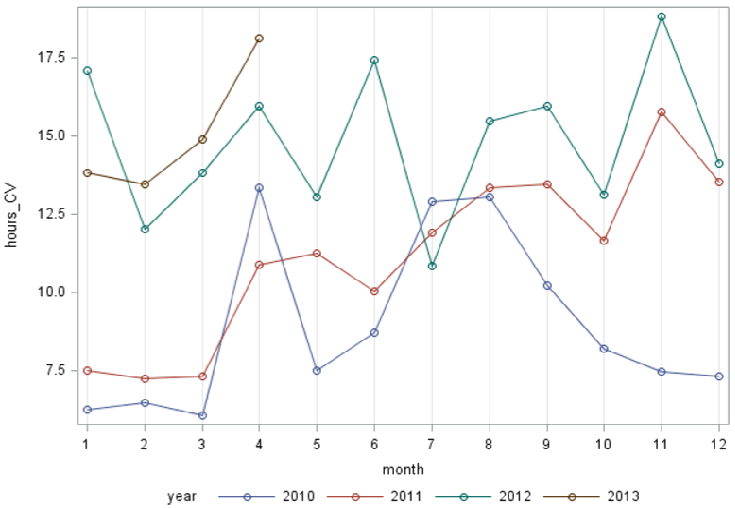
\includegraphics[width=\textwidth]{Images/CV_by_year-timeseries.png}
\caption{CV, yearly.}\hrule
\label{fig:cv}
\end{figure*}
The continuous plot, Figure~\ref{fig:cv_cont} shows that the size of the peaks and troughs does not seem to change with changing trends: the additive model is thus selected. The SAS procedure X12 agrees with that assessment, and further suggests no data transformation.
\begin{figure*}[t]
\centering
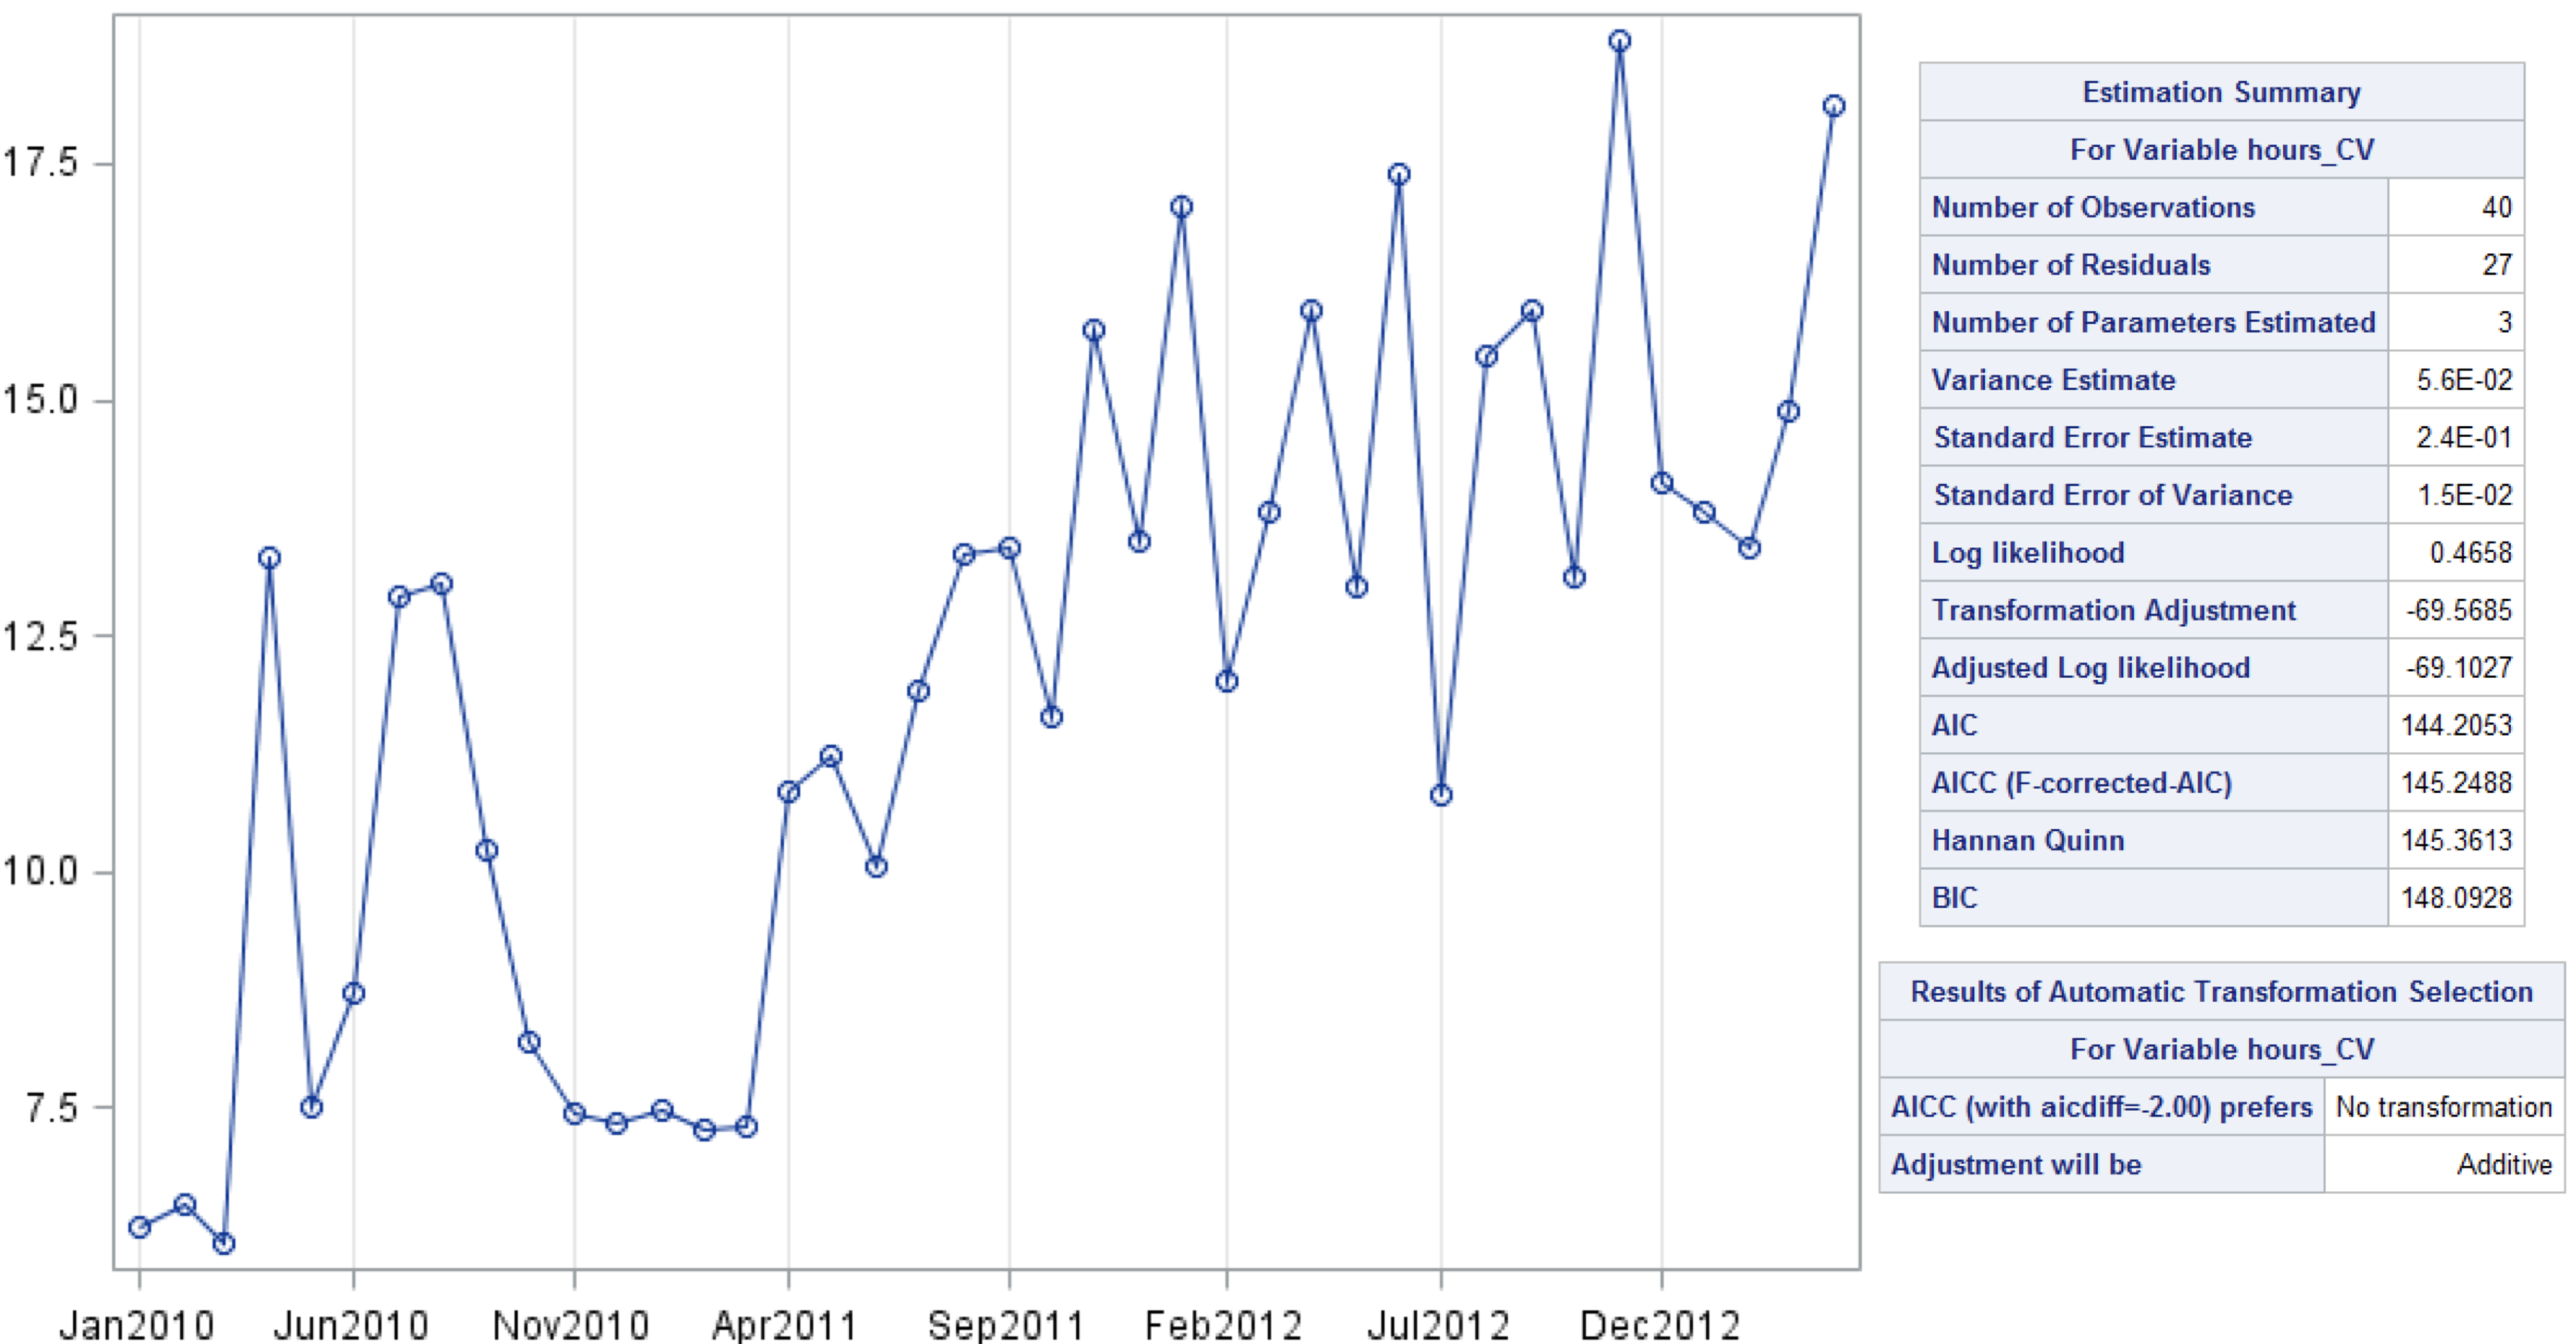
\includegraphics[width=\textwidth]{Images/CV_continuously.png}
\caption{CV, continuously; estimation summary.}\hrule
\label{fig:cv_cont}
\end{figure*}
The diagnostic plots are shown in Figure~\ref{fig:diff}: the 2010 CV series is prior-adjusted from the beginning until OCT2010 after the detection of a level shift. The SI (Seasonal-Irregular) chart shows that there are more than one irregular component which exhibits volatility.
\begin{figure*}[t]
\centering
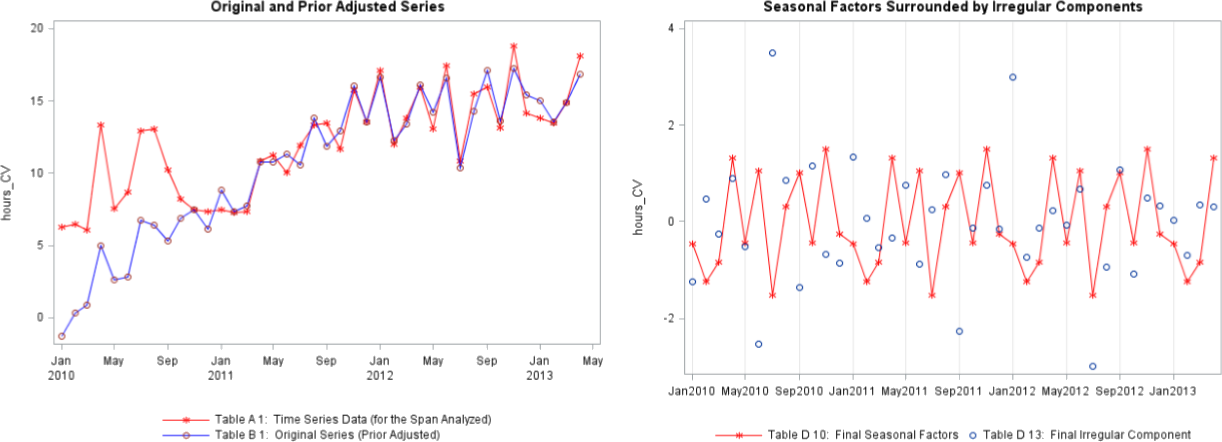
\includegraphics[width=0.98\textwidth]{Images/DiffComponents.png}
\caption[Diagnostic plots.]{Diagnostic plots. Note here that the analysis of a time series starts with estimation of the effects of festivals and trading days. These precalculated
estimates are then used for prior adjustment of the series. The prior adjusted original series is
subsequently analyzed using the seasonal adjustment.}
\label{fig:diff}
\end{figure*}
The adjusted series is shown below in Figure~\ref{fig:adjusted} (the trend and irregular components are shown separately for readability).
\begin{figure*}[t]
\centering
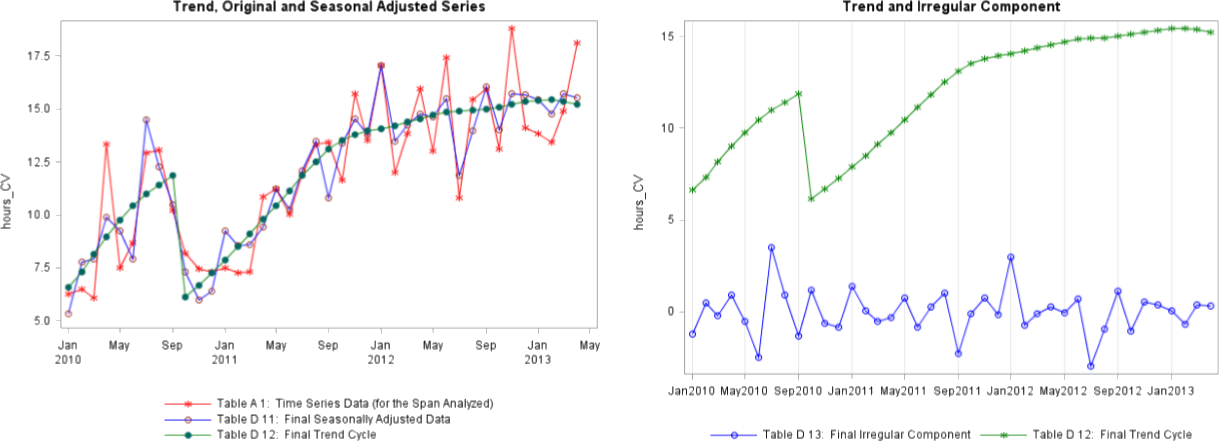
\includegraphics[width=0.98\textwidth]{Images/adjustedplot.png}
\caption{Adjusted plots}\hrule
\label{fig:adjusted}
\end{figure*}
\newl Traditionally, decomposition follows one of three models: multiplicative, additive, and pseudo-additive. 
 \begin{itemize}[noitemsep]      
    \item \textbf{Multiplicative} -- This modeling approach assumes that a) the magnitude of the seasonal spikes/troughs increases when the trend increases (and vice versa); b) the trend $T_t$ has the same dimensions as the original series $O_t$, and the seasonal component $S_t$ and the irregular component $I_t$ are dimensionless and centered around 1; c)  the seasonal fluctuation  $\sum_{j=1}^{n} S_{t+j}=0 $, where $n = 365$ for daily series, $n=12$ for monthly series,$n=4$ for quarterly series,etc.,and d) the original series $O_t$ does not contain zero values. Mathematically, the model is expressed as:
    \begin{equation*}
        O_t = T_t \times S_t \times I_t
    \end{equation*}
   All components share the same units. After seasonality adjustment, the seasonality adjusted series is
   \begin{equation*}
       SA_t = \frac{O_t}{S_t} = T_t \times I_t
   \end{equation*}
   To transfer multiplicative to additive model, we could take a logarithm transformation, such as:
   \begin{equation*}
       \log{O_t} = \log{T_t}+\log{S_t}+\log{I_t}
   \end{equation*}
    \item \textbf{Additive} -- This modeling approach assumes that: a) the seasonal component $S_t$ and the irregular component $I_t$ are independent of the trend behaviour $T_t$; b) the seasonal component $S_t$ remains stable from year to year; and c) the seasonal fluctuation $\sum_{j=1}^{n} S_{t+j}=0 $, where $n=365$ for daily series, $n=12$ for monthly series, $n=4$ for quarterly series, etc. Mathematically, the model is expressed as:
    \begin{equation*}
        O_t = T_t + S_t + I_t
    \end{equation*}
    All components share the same dimensions and units. After seasonality adjustment,the seasonality adjusted series is:
    \begin{equation*}
        SA_t = O_t - S_t = T_t + I_t
    \end{equation*}
    \item \textbf{Pseudo-additive} -- This modeling approach assumes that some of the values of the original series $O_t$ are 0 (or very close to 0) and that a) the seasonal component $S_t$ and the irregular component $I_t$ are both dependent on the trend level $T_t$, but independent of each other, and b) the trend $T_t$ has the same dimensions as the original series $O_t$, and the seasonal component $S_t$ and the irregular component $I_t$ are dimensionless and centered around 1.  Mathematically, the model is expressed as:
    \begin{equation*}
       O_t = T_t + T_t \times (S_t-1) + T_t \times (I_t -1)=T_t \times (S_t +I_t -1)  
    \end{equation*}
    All components share the same units. After seasonality adjustment, the seasonality adjusted series is:
    \begin{equation*}
        SA_t = O_t - T_t \times (S_t -1 )-T_t \times (D_t -1) = T_t \times I_t
    \end{equation*}
    \item \textbf{How to choose the model?} -- The choice of a model is driven by data behaviour and choice of assumptions. The analyst needs to plot the time series graph and test a range of models, selecting the one which stabilized the seasonal component.
    \item \textbf{Suggested methods of estimating if a time series is multiplicative, additive or pseudo-additive?} -- The simplest way to determine whether to use multiplicative or additive decomposition, is by graphing the time series. If the size of the seasonal variation increases/decreases over time, multiplicative decomposition should be used. On the other hand, if the seasonal variation seems to be constant over time, additive model should be used. A pseudo-additive model should be used when the data exhibits the characteristics of the multiplicative series, but parameter values are close to zero.
    \item \textbf{how to automate the selection of multiplicative, additive, pseudo-additive model?} -- Complete automation of the model selection will be very difficult (as there is no prior knowledge about the shape of the data). Under the assumption that the data behaves nicely, one may be able to test whether the magnitude of seasonal variability remains constant over time. Suppose that there is data from January 2010 to December 2015: if the magnitude remains constant, the ratio of seasonal component over time should be one. Comparing data points from January 2010, 2011, ..., 2015, the ratios of January 2011/January 2010, January 2012/January 2010, and so on should all be one. Otherwise, Multiplicative decomposition should be used. If the multiplicative method turns out to be ineffective (since estimating a component that is virtually 0 in multiplication is unstable), a pseudo-additive model may be chosen.
    
    
\end{itemize}



\subsection{Notes, Challenges and Pitfalls}
 \begin{itemize}[noitemsep]
\item Time series are said to be (weakly) \textbf{stationary} when time series values are independent of time (i.e. the mean and variance are stable over time). Autocorrelation function (ACF) and Partially ACF (PACF) are commonly used to determine whether a time series is stationary. The explanation is very straightforward, as shown in Figure~\ref{fig:ACF}. The lower ACF is the desired plot, implying the time series is stable. When the empirical data's ACF does not match the model's ACF, the model being considered is unlikely to be adequate. For example, if a model (such as SARIMA) is fitted, then the residuals should exhibit the ACF of a white noise series (i.e., the residuals are uncorrelated.) If the ACF/PACF show some spikes in the resulting residuals, it is an indication that the fitted model is missing some components (hence inadequate).
\item In order to identify correlations and root causes \textit{via} analysis of the relationships between the variables, one must assume that the time series values are stationary. Statistical tools which assume data independence are invalidated if the data is not actually independent of time, that is if it is \textbf{serially dependent}. Classical statistical methods are built on the assumption of independence of data points (y1, y2, ...). If they are dependent of each other (in the form of time or others), then the fundamental assumption fails, and hence these statistical methods must be adjusted for time dependence.
\begin{figure*}[t]
\centering
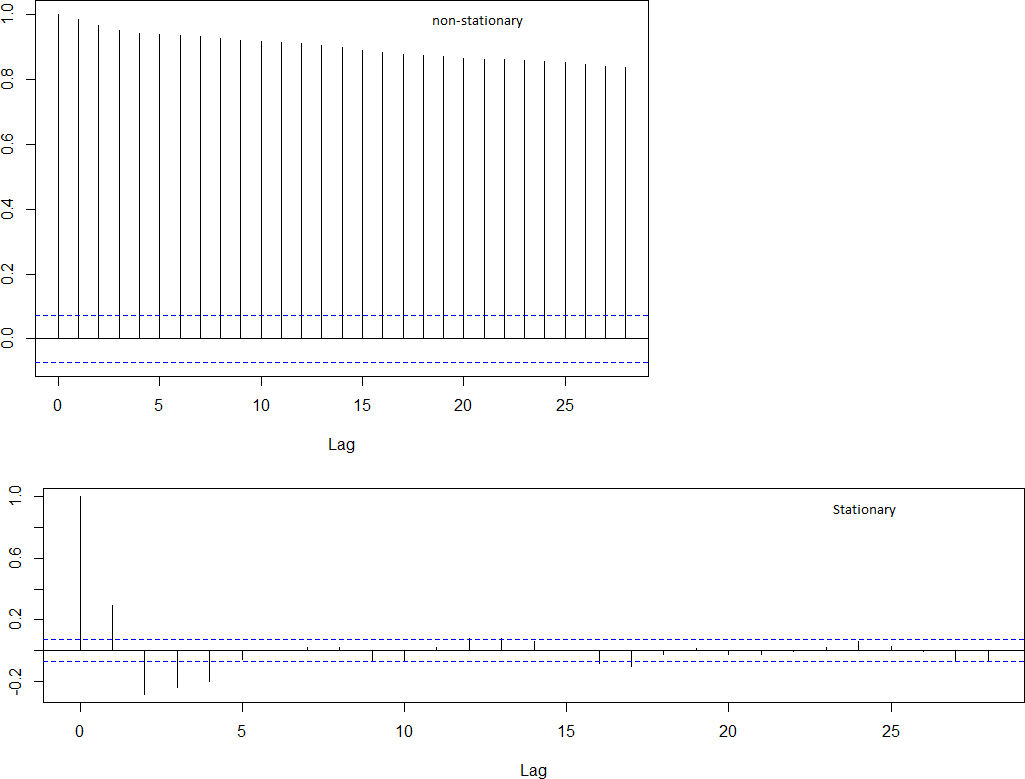
\includegraphics[width=0.90\textwidth]{Images/ACF_example.png}
\caption{ACF plots for a model which is not matching the empirical data.}\hrule
\label{fig:ACF}
\end{figure*}
\item When \textbf{non-stationary} serial dependence is suspected or expected to exist, \textbf{time series decomposition} is required to extract the data's \textbf{trend}, \textbf{cyclical}  and \textbf{seasonal components}, \textbf{calendar effects}, and \textbf{structural breaks}, in addition to providing accurate forecasts. The time series seasonal adjustment enables the identification of \textbf{turning points} and provides consistent comparisons of indicators across time periods.
\item Traditionally, time series decomposition is built on one of three models: \textbf{multiplicative}, \textbf{additive}, or \textbf{pseudo-additive}. The choice of a model is driven by data behaviour and choice of assumptions.
\item Time series decompositions, and hence any activity depending on them (such as forecasting, for instance), \textbf{ultimately rely on the quality of the underlying data}. In particular, there are a number of well-known data quality issues which affect the results of the analysis: 
\begin{enumerate}
\item the method of data collection may lead to unusual effects, especially if collection is made on a non-calendar basis or if there is a lag between activity and measurement;
\item any change to the method or timing of data collection could lead to the false identification of trend or seasonal breaks;
\item some series are sensitive to events such as extreme weather, strikes, wars, etc., which could cause breaks or outliers of large magnitude;
\item at least 5 years' worth of data are required to insure stability on future updates, and
\item at least 10 years' worth of data are required to insure that the adjustment of the first year is unlikely to be revised.    
\end{enumerate}
\item Forecasts tend to be \textbf{wrong}: aggregated forecasts (using more than one model and aggregating the results, instead of using a single model) are usually more accurate. Emphasis should not be placed on a \textbf{single estimate} (such as the mean): they should also include the \textbf{standard deviation} or an \textbf{accuracy range}.  
\item Identification of trend in time series is subjective because what appears to be a trend over a short time period may prove to simply be a \textbf{small fluctuation} which could form part of a cycle over the long-term horizon of the series. 
\item Regression models of various complexity levels can be fitted (against time and/or auxiliary variables) to identify possible trends. At long horizons, polynomial response functions explode: if such models must be used, \textbf{it is recommended to use linear or quadratic response functions}, as slope and concavity might be the best we can hope to detect in light of the previous remark. 
\item In combination with \textbf{appropriate data transformations} (e.g. logarithm, square root, inverse, Box-Cox, etc.), low order regression models can achieve good results. 
\item \textbf{power transformation} is the simple and effective way to stabilize the variances, including square root, cube root, logarithm, etc.
\item \textbf{Fourier transforms} can help identify potential trend and cycles (as well as their respective frequencies), so can a variety of statistical tests (like the \textbf{Mann-Kendall} test, for instance). 
\item De-trending methods come with strengths and weaknesses:
\begin{enumerate}
\item \textbf{Finite Differences} are iterated differences between subsequent time series observations, which can remove polynomial trends. They are useful if the exact shape of trend cannot be estimated, but too high an order may introduce variance inflation. They ignore the potential effect of any variable over the trend, save for the passage of time.
\item \textbf{Curve Fitting} includes regressions against time as well as more complicated models involving auxiliary variables. Prior knowledge of the situation under consideration can be used to provide an acceptable model which na\"{\i}ve analysis of the data might not be able to suggest,  but a  simple regression model may be unrealistic. 
\item \textbf{Filtering and Smoothing} consists of various weighted averages of the time series data which are used to compute a filtered series. Their advantages and disadvantages are discussed below. Note that filtering and smoothing methods preclude the possibility of finding an explicit functional form for the trend.
\begin{description}
\item[Moving average of order $N$] is the arithmetic average of the most recent $N$ observations. It tends to provide \textbf{stable forecasts}, and bad data (e.g. irregular points, bad stretches) is \textbf{eventually removed} from the prediction process; however, it requires saving a potentially large number of past data points, it can \textbf{lag} behind the actual trend, and it ignores complex relationships in data.
\item[Weighted moving average of order $N$] attaches importance to certain observations in the form of weights (recent observations could have more influence than older observations, for example); such weighted average may \textbf{reduce the lag} behind the trend, but there's no natural and universal way to select the weights.
\item[Exponential Smoothing] is a weighted moving average with declining weights for past data which carries the entire past history of the series, without the need to save past data points. They tend to produce \textbf{stable forecasts}, but may \textbf{increase the lag}.
\item[Holt's Method] is a double exponential smoothing which allows for quick multi-step forecasts in the presence of linear trend.
\item[Winter's Method] is a triple exponential smoothing with can take seasonal factors into consideration. At least two complete data cycles are required to provide initial estimates, and a third cycle is required for fine-tuning.  
\end{description}
\item \textbf{Cubic Splines} fit the data to a sequence of separate cubic polynomials for every sequence of three points in the series (the first and second derivatives are continuous at each point, ensuring a well-behaved curve). A parameter has to be specified which depends on the relative importance given to ``smoothness'' and ``goodness-of-fit'' of the spline. These methods are prone to overfitting the data. 
\end{enumerate}
\end{itemize}

\subsection{Non-Linear Models}
Linear models are not always appropriate to describe the data. In this section, we introduce two (of many) potential non-linear models: TAR (Threshold Autoregressive) and GARCH.
Non-parametric models allow data to have different states or regimes, and models to be dynamic in these different regimes. 
\newl Threshold autoregression is the extended application of the autoregressive model (AR), defined as 
\begin{equation*}
y_t = \beta^{(1)}_0 + \beta^{(1)}_1y_{t-1}+ \epsilon_t\quad \text{if }y_{t-1} \leqslant \gamma; 
\end{equation*}
\begin{equation*} 
y_t = \beta^{(2)}_0 + \beta^{(2)}_1y_{t-1}+ \epsilon_t\quad \text{if }y_{t-1} > \gamma.
\end{equation*}
where $\beta^{(1)}$ and $\beta^{(2)}$ are less than 1; $\epsilon_t$ is the error term; $\gamma \in \mathbb{R} $. There is one model for
each side of the threshold. Without two different models, this is simply an AR model.
The above equation is a simple example of the TAR model and in general, analysts could set different thresholds. When the threshold $ \gamma = y_{t-d} $, with a delayed parameter $d>0$, the TAR model is called self-exciting TAR or SETAR. 
\newl An autoregressive conditionally heteroscedastic (ARCH) model is used to model a changing variance per time period, and in most cases, it is used when increased variation occurs in short periods. Applications are common in economic and financial domains. The GARCH model is the generalized version of the ARCH model; GARCH(1,1), for instance, looks like:
\begin{equation*}
    \sigma^2 = \alpha_0 + \alpha_1 y^2_{t-1} + \beta_1 \sigma^2_{t-1}.
\end{equation*}
The initial step of finding the ``correct'' model is to plot the time series and, depending on the properties of the plot, to set up up parameters and candidate models. For instance, to identify which ARCH model would be ideal, one could look at the autocorrelation function plots of $y_t$ and $y^2_t$ -- an ARCH(1,1) model would be appropriate if $y_t$ seems to be a white noise and $y^2_t$ follows an AR(1) model. Other tests exist (see Shumway and Stoffer's \textit{Time Series Analysis and its Applications} for more examples). 

\section{Results Evaluation}
In the previous sections, we have discussed how to select parameters and generate models. The next task is to evaluate the models: to apply the candidates to the data and compare their results. Evaluation measures the ``difference'' between estimated and true values (the residual). Usually, analysts separate the data into training and testing sets, retaining a small portion for the purpose of validation. The optimal model parameters include the Akaike Information Criterion (AIC) and the Bayesian Information Criterion (BIC). The two parameters measure not only the goodness-of-fit of a model, but also its simplicity. Generally speaking, the lower AIC/BIC a model possesses, the better the model would be, but the value in isolation is of little use. Furthermore, the performance of forecasting on the training data can also be evaluated by model forecasting accuracy matrices (such as a confusion matrix). The criteria are defined as follows:
\begin{equation*}
\mathrm{AIC}(p)=n \ln(\sigma^2_e/n)+2p 
\end{equation*}
\begin{equation*} 
\mathrm{BIC}(p)=n \ln(\sigma^2_e/n)+p+p \ln(n)
\end{equation*}
where $p$ is the number of the parameters in the model, $n$ is the number of observations, and $\sigma^2_e$ is the sum of squared residuals using the fitted time series given by the model . 
\newl Other approaches also exist. Let $y_t$ denote the actual value of the time series, $\hat{y_t}$ be its forecast, and $e_t=y_t-\hat{y_t}$ be the error.
 \begin{itemize}[noitemsep]
\item \textbf{The Mean Forecast Error (MFE)} is defined as $\mathrm{MFE}=\frac{1}{n} \sum_{t=1}^{n} e_t $ where $n$ is the number of observations. Clearly, a desired MFE will be close to zero. Even though it is easy to compute, it has many disadvantages: an MFE near 0 does not necessarily lead to good forecasts due to positive and negative errors potentially cancelling out; the MFE is easily affected by extreme values, and it is unduly influenced by data transformations. Similarly, the \textbf{mean absolute error} (MAE) and the \textbf{mean absolute deviation} (MAD) measure the average absolute difference between forecasts and the real values. Unlike MFE, MAE takes into account the magnitude of overall error. 
\item \textbf{The Mean Absolute Percentage Error (MAPE)} is given by, $ \mathrm{MAPE}=\frac{1}{n} \sum_{t=1}^{n} \frac{\left|e_t\right|}{\left|y_t\right|} \times 100 $, which measures the percentage of average absolute error. MAPE is independent of the scale; but it is unduly affected by data transformation and extreme cases, and opposite errors cancel out.
\item \textbf{The Mean Squared Error (MSE)} $= \frac{1}{n} \sum_{t=1}^n {e^2_t}$ measures the average squared deviation of the forecast. Mathematically, a squared root version of MAPE is given by $$\mathrm{RMSE}=\sqrt{\mathrm{MSE}}=\sqrt{\frac{1}{n} \sum_{t=1}^{n} e^2_t}.$$ Unlike MAPE, $y_t$ being zero or very small does not affect the MSE much, but MSE measurement is not scale-free. 
\item \textbf{The Normalized Mean Squared Error (NMSE)} is defined as $$\mathbf{NMSE} =\frac{MSE}{\sigma^2}=\frac{1}{\sigma^2 n} \sum_{t=1}^{n} e^2_t,$$ which normalizes the MSE. It has similar properties to the MSE, but is more effective. The smaller the NMSE of a model is, the better the forecast will be. 
\item \textbf{Theil's U-statistic} is given by $$ U=\frac{\sqrt{\sum_{t=1}^{n} e^2_t /n}}{\sqrt{\sum_{t=1}^{n} \hat{y}^2_t /n \sqrt{\sum_{t=1}^{n} y^2_t /n}}}.$$ It compares the actual values with the results of forecasting with historical data. Due to the squared value, large errors have more weights. Its interpretations are that if $U<1$, then the forecast is better than mere guessing; if $U=1$, there is no difference; if $U>1$, then the forecast is worse than guessing, and if $u=0$ the fit is near perfect. 
\end{itemize}
We have presented some selected metrics to evaluate the forecasting results and each of them has its own set of properties. In practice, a model's validity is gauged by looking at more than one metric, in order to mimize the odds of making a mistake. 
\section{Case Study: Multi-Modal Supply Chains} What can we say about this project? \newpage\newpage
\setboolean{@twoside}{false}

\includepdf[pages={1-6},offset={0 0}]{Images/Summary_TC.pdf}
\setboolean{@twoside}{true}